\begin{figure}
    \centering
    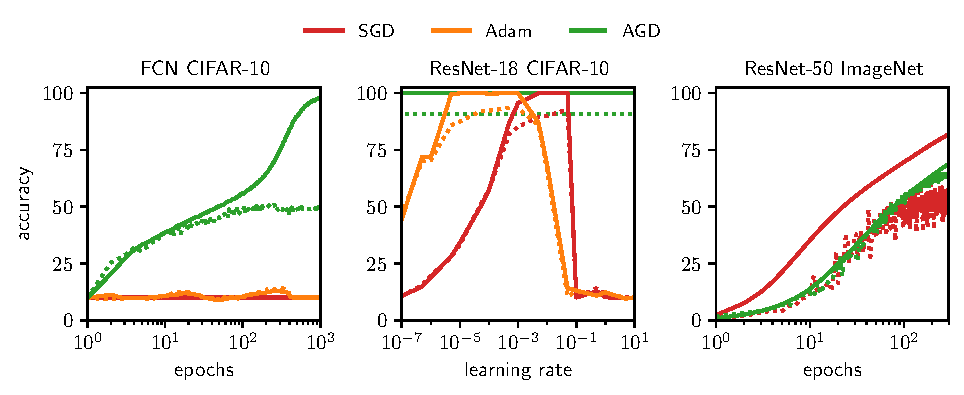
\includegraphics[width=\textwidth]{figures/pdf/plot0}
    \caption{\captiontitle{Automatic gradient descent trains neural networks reliably without hyperparameters.} Solid lines show train accuracy and dotted lines show test accuracy. The networks are unregularised with biases and affine parameters disabled, as these features are not yet supported by AGD. In the \captiontitle{left panel}---unlike AGD---Adam and SGD failed to train a 32-layer fully-connected network on CIFAR-10 with their default learning rates of 0.001 for Adam and 0.1 for SGD. The \captiontitle{middle panel} displays a learning rate grid search for ResNet-18 trained on CIFAR-10. AGD attained performance comparable to the best tuned performance of Adam and SGD. In the \captiontitle{right panel}, AGD trained ResNet-50 on ImageNet to a top-1 test accuracy of 65.5\%. The ImageNet baseline is SGD with a learning rate of 0.1 and no learning rate decay schedule.}
    \label{fig:showcase}
\end{figure}